% Compatibilidad con instalaciones MiKTeX cuyo formato base es anterior a
% la versión instalada de Hyperref.
\providecommand{\IfFormatAtLeastTF}[3]{#3}
\providecommand{\IfFormatAtLeastT}[2]{}
\providecommand{\IfFormatAtLeastF}[2]{#2}
\providecommand{\IfDocumentMetadataTF}[2]{#2}
\providecommand{\IfDocumentMetadataT}[1]{}
\providecommand{\IfDocumentMetadataF}[1]{#1}

\documentclass[11pt]{article}

\usepackage[T1]{fontenc}
\usepackage[utf8]{inputenc}
\usepackage[spanish,es-nodecimaldot]{babel}
\usepackage{lmodern}
\usepackage[margin=1in]{geometry}
\usepackage{amsmath,amssymb}



\usepackage{graphicx}
\graphicspath{{Figuras/}}



\setlength{\parindent}{0pt}
\setlength{\parskip}{0.45em}
\renewcommand{\labelenumi}{\textnormal{(\alph{enumi})}}
\pagestyle{plain}

\let\enumerateoriginal\enumerate
\let\endenumerateoriginal\endenumerate
\renewenvironment{enumerate}{%
  \enumerateoriginal
  \setlength{\itemsep}{0.5em}%
  \setlength{\parsep}{0pt}%
  \setlength{\topsep}{0.4em}%
}{\endenumerateoriginal}

\newcounter{problema}
\newenvironment{problema}[1]{%
  \par
  \refstepcounter{problema}%
  \addvspace{0.9em}%
  \noindent\textbf{Ejercicio \theproblema. #1}
  \par\nobreak\smallskip
}{\par}

\begin{document}

\begin{center}
  {\large\textbf{Centro de Investigación y Docencia Económicas}}\\[0.25em]
  {\large\textbf{Macroeconomía II}}\\[0.2em]
  {\large\textbf{Problem Set 4: Dinero, Banca, Precios y Política Monetaria} \\
  Solver}\\[0.35em]
  LECO -- Otoño 2026
\end{center}

\vspace{0.6em}

\textbf{Ejercicio 1.} El gobierno decide que el uso de tarjetas de crédito es perjudicial e introduce un impuesto sobre los saldos en tarjetas de crédito. Es decir, si un consumidor o empresa mantiene un saldo de tarjeta de crédito igual a \(X\) en términos reales, paga un impuesto de \(tX\), donde \(t\) es la tasa impositiva. Determine los efectos de esta medida sobre el precio y la cantidad de equilibrio de saldos de tarjetas de crédito, la demanda de dinero y el nivel de precios. Explique sus resultados.

\vspace{0.5em}

\textbf{Ejercicio 2.} En el modelo monetario intertemporal, suponga que entra en operación una nueva innovación tecnológica que incrementa permanentemente la productividad total de los factores. Determine los efectos presentes sobre la producción agregada, el consumo, la inversión, el empleo, el salario real, la tasa de interés real, la tasa de interés nominal y el nivel de precios, bajo los siguientes escenarios:

\begin{enumerate}
    \item El efecto sobre la tasa de interés real provocado por el choque en la oferta de producto asociado con la mayor productividad presente domina al efecto del choque en la demanda de producto originado por la mayor productividad futura.

    \item El efecto sobre la tasa de interés real provocado por el choque en la demanda de producto asociado con la mayor productividad futura domina al efecto del choque en la oferta de producto originado por la mayor productividad presente.

    \item Ambos efectos sobre la tasa de interés real se compensan exactamente.

    \item Suponga que el banco central conduce la política monetaria bajo un régimen de metas de inflación, con una meta de $\pi^*=0$, utilizando la oferta monetaria como instrumento de política. ¿Cómo debe ajustar la oferta monetaria ante cada uno de los escenarios anteriores para cumplir con su objetivo? Explique.

    \item Suponga ahora que el banco central utiliza la tasa de interés nominal como objetivo operativo de política monetaria, manteniendo la misma meta de inflación. ¿Cómo debe ajustar la tasa de interés nominal ante cada uno de los escenarios anteriores para cumplir con su objetivo? Explique.

\end{enumerate}



\subsubsection*{Solución}
Los efectos reales son los mismos que los analizados en el modelo intertemporal del sector real. Dado que en este modelo se cumple la dicotomía clásica, podemos primero desglosar los efectos sobre variables reales y después determinar los efectos sobre las variables nominales.

\paragraph{Inciso (a).} La figura~\ref{fig:1.a} muestra el mecanismo neto. Los desplazamientos en azul representan los efectos de equilibrio del incremento en la productividad presente, mientras que los desplazamientos en rojo incorporan adicionalmente los efectos del aumento en la productividad futura.

\begin{figure}[htbp]
    \centering
    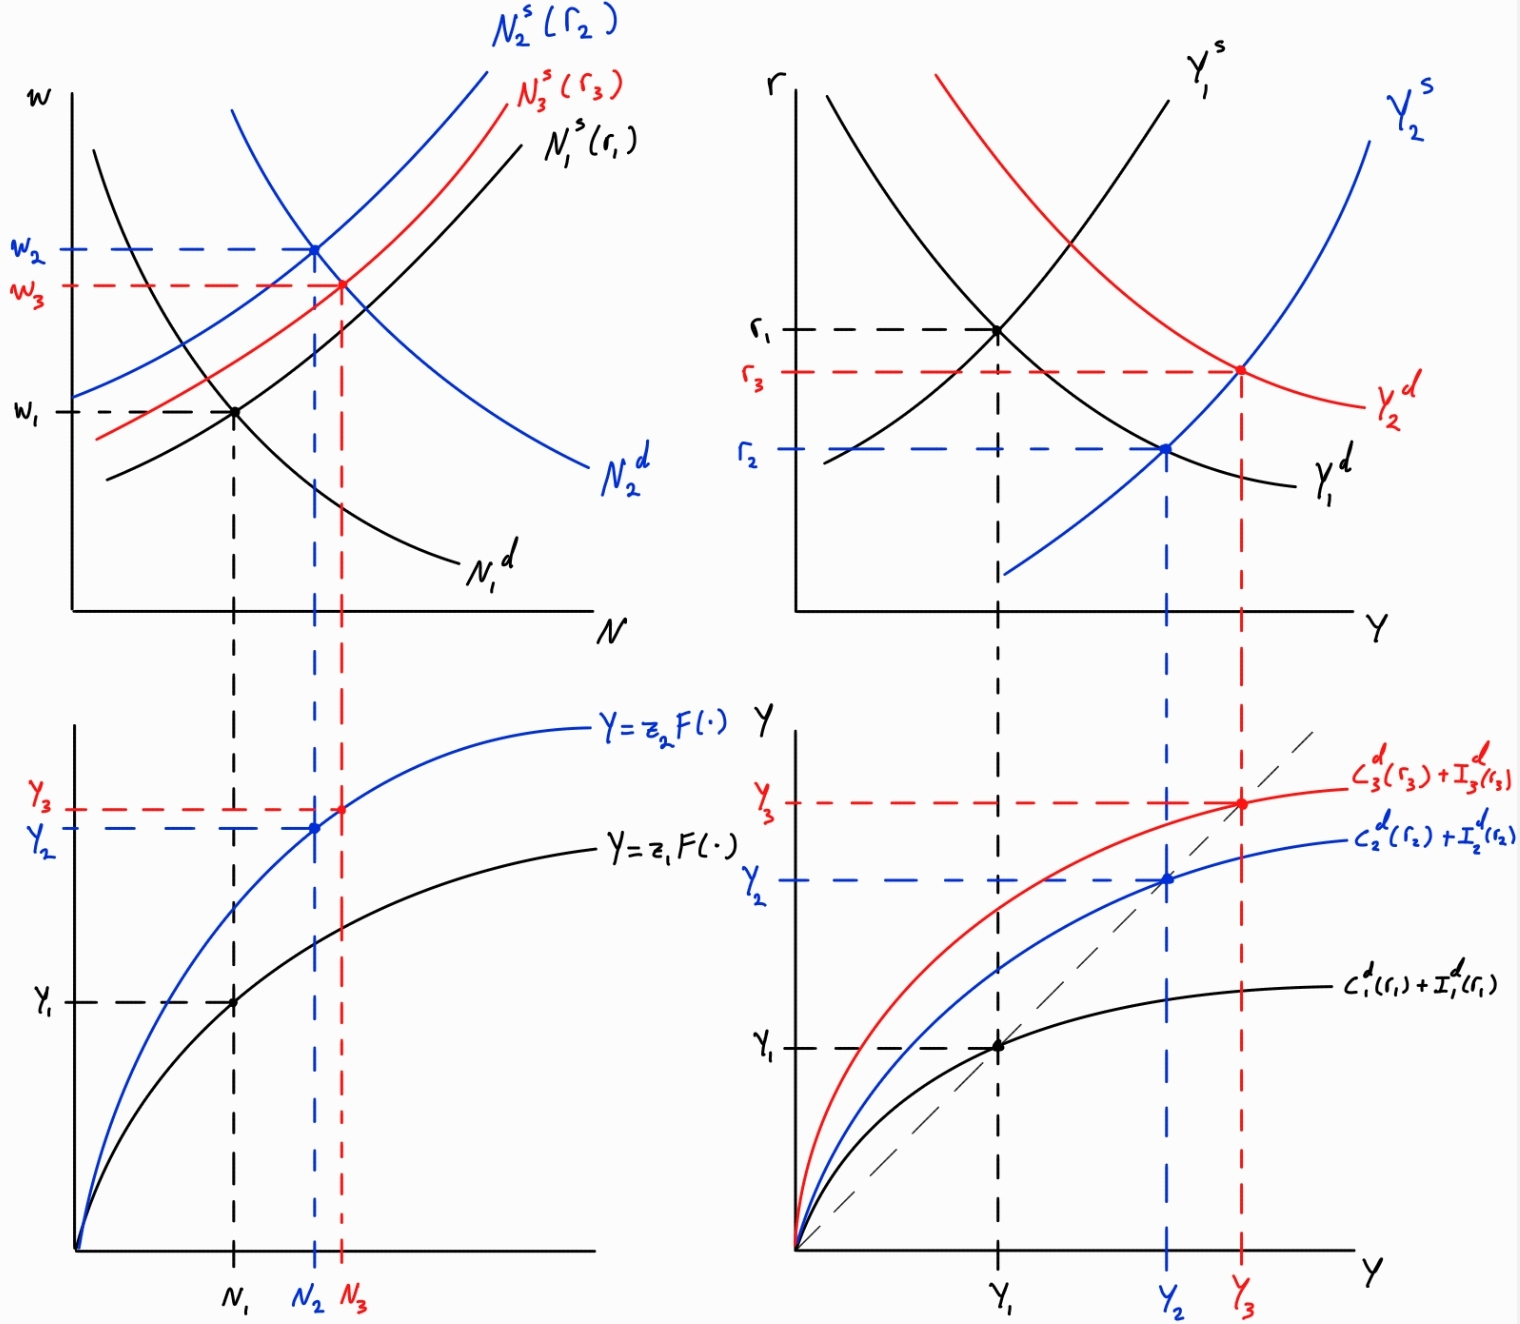
\includegraphics[width=0.95\textwidth]{a.jpg}
    \caption{Efectos de un choque permanente de productividad: Caso (a)}
    \label{fig:1.a}
\end{figure}


\paragraph{Efectos del incremento en la productividad presente.}
El aumento en $z$ eleva el producto marginal del trabajo, generando incentivos a contratar más trabajadores. Esto desplaza hacia la derecha la curva de demanda laboral. Simultáneamente, la mayor productividad desplaza hacia arriba la función de producción, pues le permite a la empresa representativa producir una mayor cantidad de bienes y servicios para cualquier nivel de empleo. Ambos efectos se traducen en un incremento de la producción para cada nivel de la tasa de interés real, provocando un desplazamiento hacia la derecha de la curva de oferta agregada de bienes y servicios.

El exceso de oferta resultante en el mercado de bienes ejerce una presión a la baja sobre la tasa de interés real. Su reducción desincentiva el ahorro e incentiva el consumo presente, debido al efecto sustitución intertemporal, al tiempo que estimula la inversión al reducir su costo de financiamiento. Por otra parte, la menor tasa de interés real desincentiva la oferta laboral presente debido a la sustitución intertemporal del trabajo, desplazando la curva de oferta laboral hacia la izquierda, lo que modera el incremento inicial de la producción. En conjunto, el aumento en la demanda de consumo e inversión y la moderación de la oferta laboral se reflejan en \textbf{movimientos sobre} las curvas de demanda y oferta de bienes y servicios, hasta restablecer el equilibrio en este mercado.

Suponemos que la contracción de la oferta laboral es suficientemente pequeña para que domine el desplazamiento positivo de la demanda laboral. Bajo este supuesto, tanto el empleo como el salario real aumentan. Asimismo, el producto agregado se incrementa y la tasa de interés real disminuye, de modo que la economía pasa del equilibrio inicial a un equilibrio intermedio, representado por el subíndice $2$.

\paragraph{Efectos adicionales del incremento en la productividad futura.}
El aumento en $z'$ eleva el producto marginal esperado del capital futuro, incrementando la rentabilidad futura de la inversión presente. En consecuencia, la demanda de inversión aumenta para cada nivel de la tasa de interés real, desplazando hacia la derecha la demanda agregada de bienes y servicios.

Este desplazamiento genera un exceso de demanda de bienes al nivel de la tasa de interés real del equilibrio intermedio, ejerciendo una presión al alza sobre dicha tasa. El incremento de la tasa de interés real respecto a $r_2$ modera el incremento en la demanda de bienes y desplaza la oferta laboral presente hacia la derecha debido a la sustitución intertemporal del trabajo, hasta restablecer el equilibrio en ambos mercados.

\textbf{En este inciso}, suponemos que el efecto sobre la tasa de interés del choque de oferta de producto provocado por el aumento en la productividad presente domina al efecto del choque de demanda de producto asociado con el incremento en la productividad futura. Bajo este supuesto, la tasa de interés real de equilibrio se reduce respecto a su equilibrio inicial, de modo que $r_2<r_3<r_1$. 

Dado que la tasa de interés real final es inferior a la inicial y que la productividad futura es mayor, la inversión y el consumo necesariamente aumentan respecto al equilibrio inicial.


En el mercado laboral, suponemos que los desplazamientos de la oferta laboral inducidos por las variaciones en la tasa de interés real son relativamente pequeños y quedan dominados por el incremento en la demanda laboral derivado de la mayor productividad presente. Por lo tanto, el empleo y el salario real aumentan respecto a su equilibrio inicial, pasando de $N_1$ y $w_1$ a $N_3$ y $w_3$.

Finalmente, el incremento en la productividad presente, junto con el aumento en el empleo de equilibrio, implican necesariamente un mayor producto agregado, de modo que $Y_3>Y_2>Y_1$.



\paragraph{Inciso (b).} La figura~\ref{fig:1.b} muestra el mecanismo neto.

\begin{figure}[htbp]
    \centering
    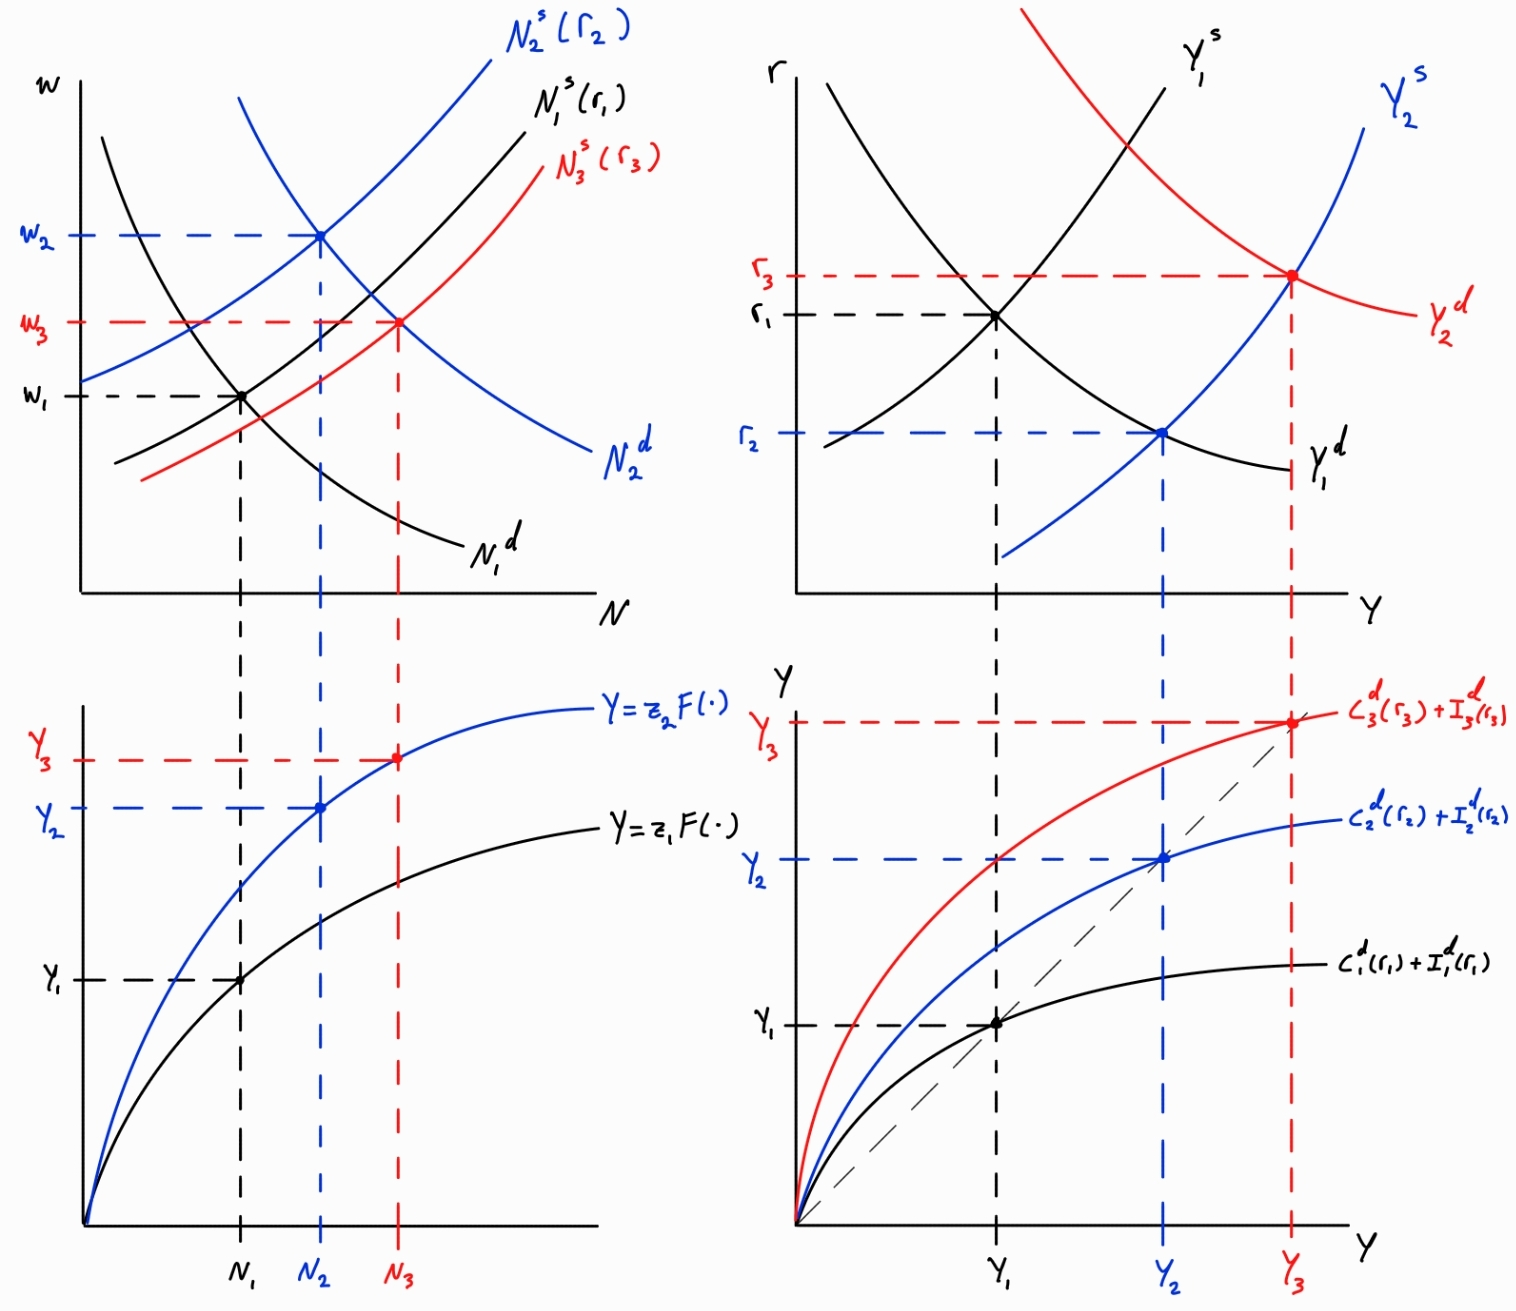
\includegraphics[width=0.95\textwidth]{b.jpg}
    \caption{Efectos de un choque permanente de productividad: Caso (b)}
    \label{fig:1.b}
\end{figure}

En este caso, suponemos que el efecto positivo sobre la tasa de interés real provocado por el desplazamiento de la curva de demanda de bienes y servicios domina al efecto negativo asociado con el desplazamiento de la curva de oferta. Es decir, el incremento en la demanda de bienes y servicios, impulsado por la mayor inversión derivada del aumento en la productividad futura, es suficientemente grande para contrarrestar el efecto a la baja sobre la tasa de interés real generado por el incremento en la oferta de producto. En consecuencia, la tasa de interés real aumenta respecto a su equilibrio inicial.

El efecto total sobre el consumo presente es ambiguo, pues operan dos mecanismos contrapuestos. Por un lado, el incremento en la productividad futura, $z'$, aumenta la riqueza intertemporal del hogar, generando un efecto ingreso positivo que incentiva el consumo presente. Por otro lado, el aumento en la tasa de interés real incentiva el ahorro y desincentiva el consumo presente mediante el efecto sustitución intertemporal. Por lo tanto, la respuesta del consumo depende de la magnitud relativa de ambos efectos.

\paragraph{Inciso (c).} La figura~\ref{fig:1.c} muestra el mecanismo neto.

\begin{figure}[htbp]
    \centering
    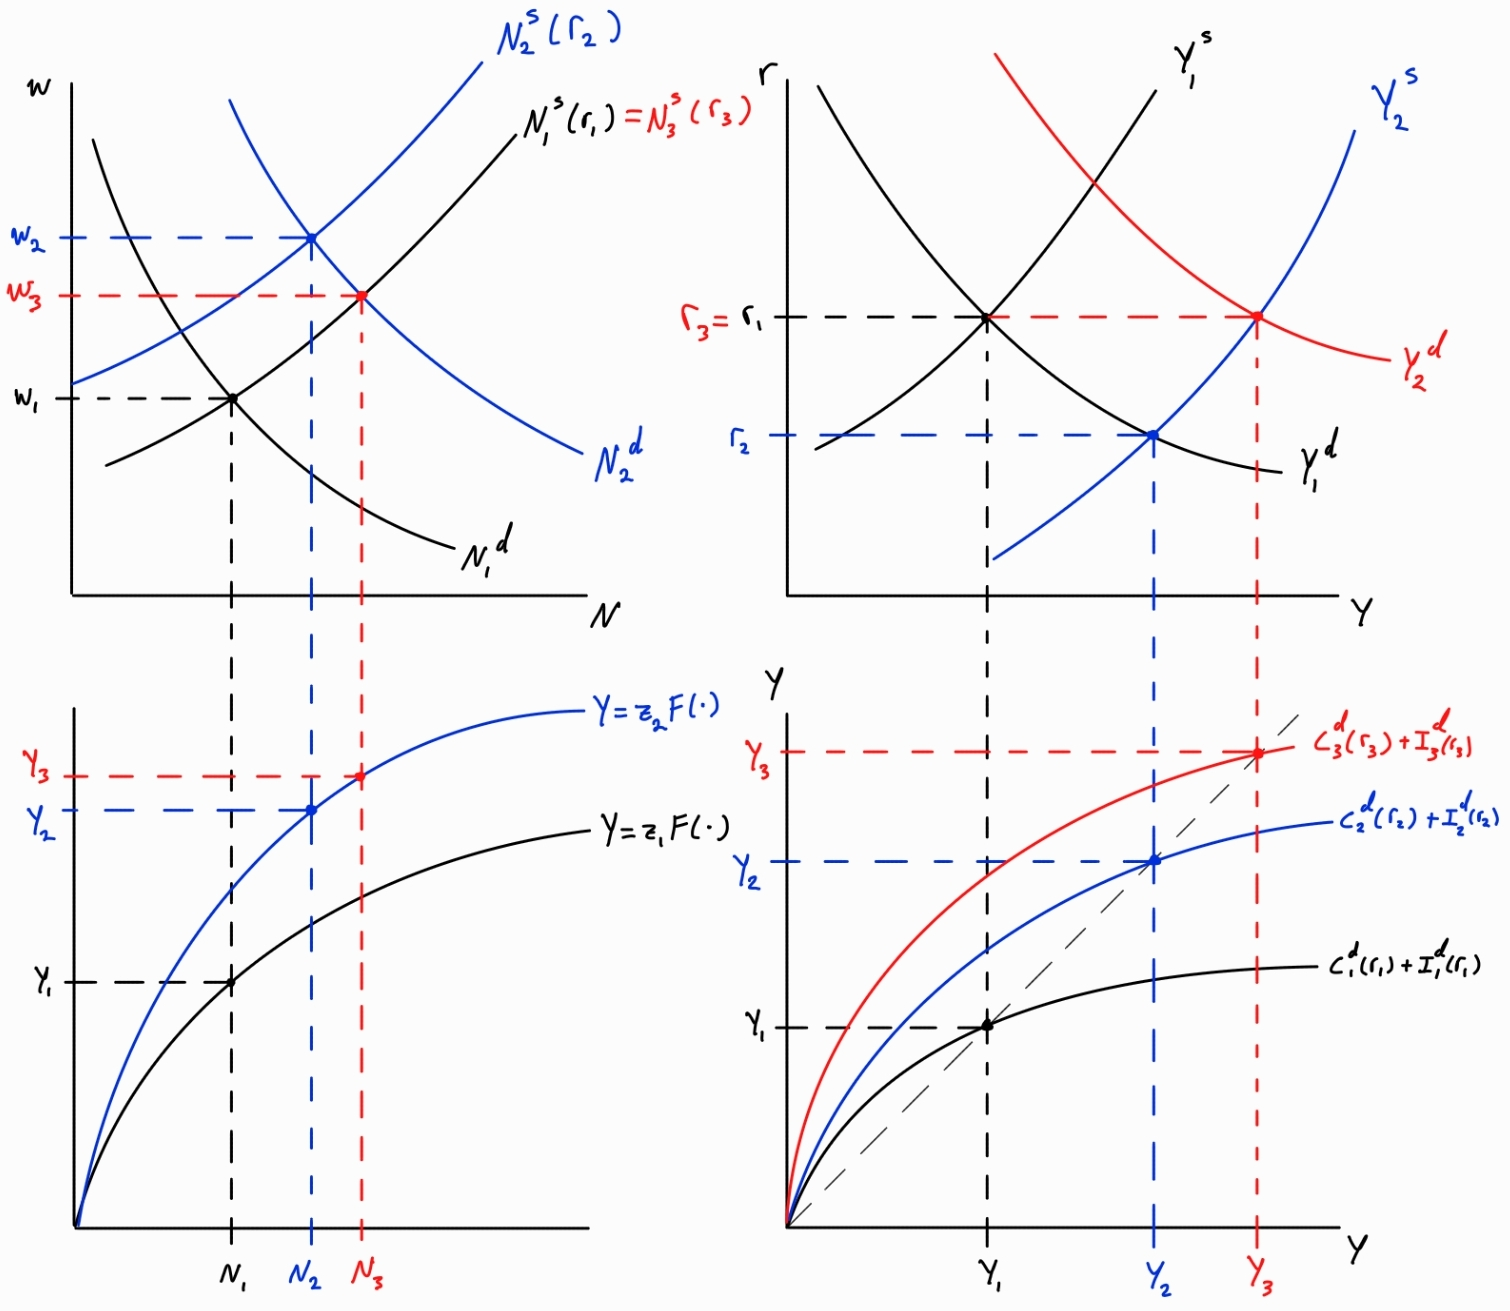
\includegraphics[width=0.95\textwidth]{c.jpg}
    \caption{Efectos de un choque permanente de productividad: Caso (c)}
    \label{fig:1.c}
\end{figure}

En este caso, suponemos que el efecto positivo sobre la tasa de interés real provocado por el desplazamiento de la curva de demanda de bienes y servicios y el efecto negativo asociado con el desplazamiento de la curva de oferta se cancelan exactamente. Es decir, el incremento en la demanda de bienes y servicios, impulsado por la mayor inversión derivada del aumento en la productividad futura, es igual efecto a la baja sobre la tasa de interés real generado por el incremento en la oferta de producto. En consecuencia, la tasa de interés real se mantiene en su equilibrio inicial.



\paragraph{Efectos sobre las variables nominales.}

Una vez analizados los mecanismos de transmisión en el sector real, podemos estudiar conjuntamente las consecuencias sobre las variables nominales en los tres escenarios. La figura~\ref{fig:1.m} ilustra los efectos sobre el equilibrio en el mercado de dinero.

\begin{figure}[htbp]
    \centering
    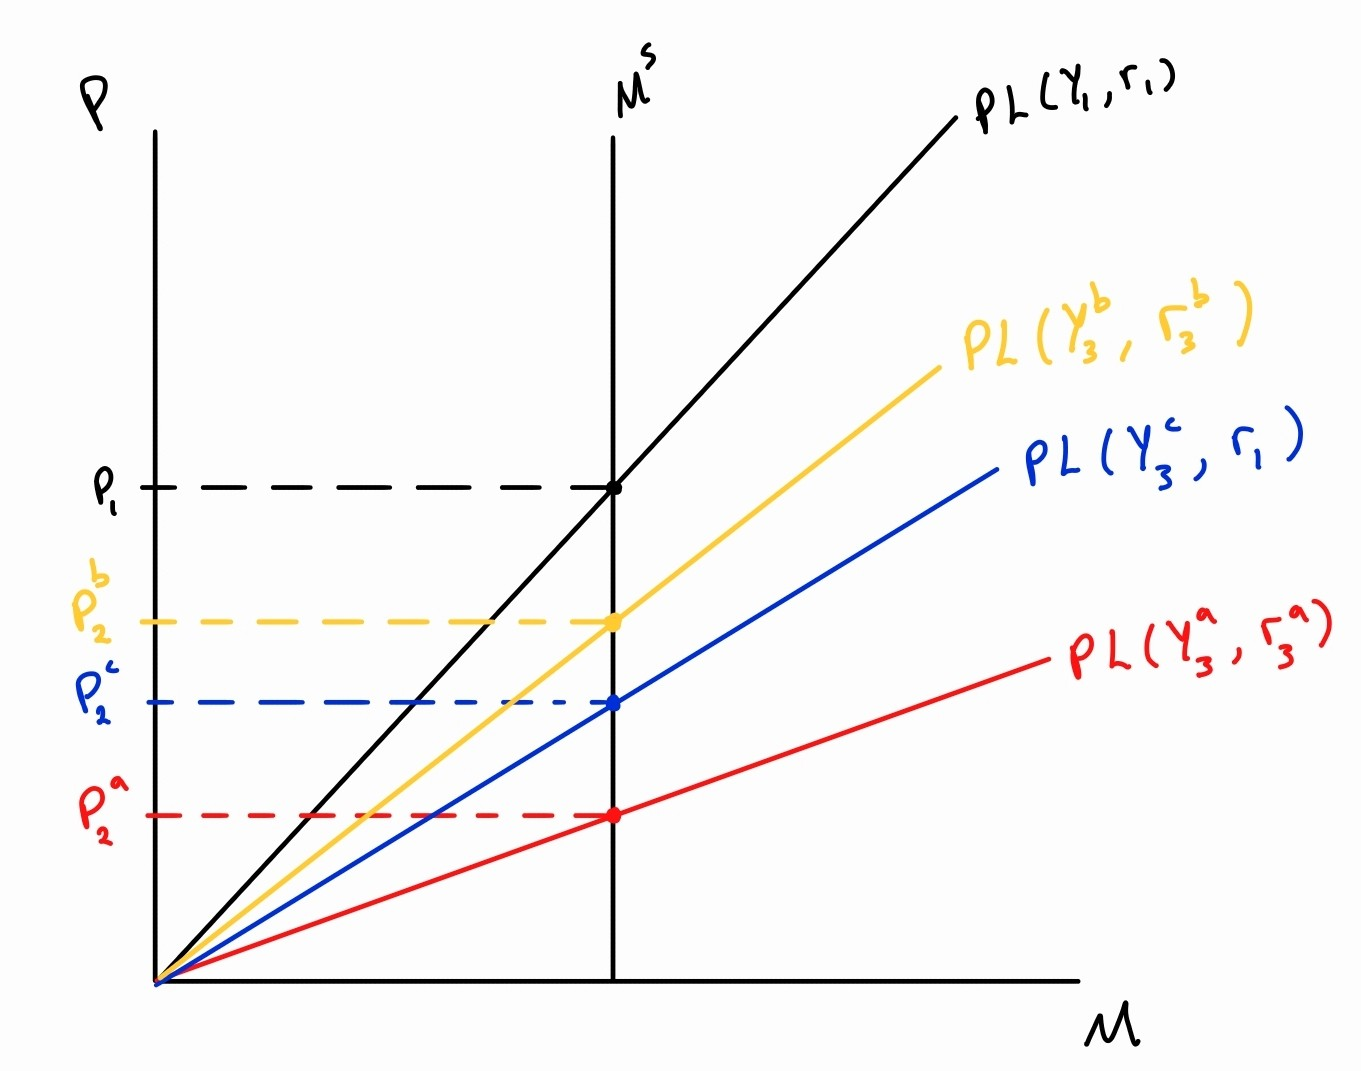
\includegraphics[width=0.7\textwidth]{m.jpg}
    \caption{Efectos sobre el equilibrio en el mercado de dinero}
    \label{fig:1.m}
\end{figure}

La demanda real de dinero, $L(Y,i)$, depende positivamente del nivel de producción agregada, debido a la mayor demanda de dinero para realizar transacciones, y negativamente de la tasa de interés nominal, que representa el costo de oportunidad de mantener dinero en efectivo.

Por la ecuación de Fisher, suponiendo que las expectativas de inflación permanecen constantes, los movimientos en la tasa de interés nominal coinciden con los de la tasa de interés real: $i = r$.

De los resultados obtenidos en el sector real, sabemos que el producto agregado aumenta en los tres escenarios. En particular, notemos que los niveles de producción de equilibrio satisfacen:
\[
Y_1<Y_3^a<Y_3^c<Y_3^b,
\]
donde $Y_3^x$ representa el producto agregado de equilibrio final en el escenario $x\in\{a,b,c\}$.

Por su parte, las tasas de interés reales de equilibrio satisfacen:
\[
r_3^a<r_3^c=r_1<r_3^b.
\]

En consecuencia, los efectos sobre la demanda real de dinero son:
\begin{align*}
    &\text{Caso (a):}\qquad
    Y\uparrow,\quad i\downarrow
    \implies L\uparrow, \\[4pt]
    &\text{Caso (b):}\qquad
    Y\uparrow,\quad i\uparrow
    \implies L\text{ ambiguo}, \\[4pt]
    &\text{Caso (c):}\qquad
    Y\uparrow,\quad i=
    \implies L\uparrow.
\end{align*}

En el escenario (a), ambos efectos incrementan la demanda real de dinero: la mayor producción eleva la demanda de dinero para transacciones, mientras que la reducción de la tasa de interés nominal disminuye su costo de oportunidad.

En el escenario (b), los efectos son contrapuestos. El aumento en la producción incrementa la demanda real de dinero, mientras que la mayor tasa de interés nominal la reduce. Por lo tanto, el efecto neto es ambiguo y depende de la magnitud relativa de ambos mecanismos. La figura~\ref{fig:1.m} muestra el caso en que el efecto del incremento en $Y$ es mayor al efecto del incremento en $i$, de modo que la demanda de dinero se desplaza hacia la derecha.

En el escenario (c), la tasa de interés nominal permanece constante, por lo que el incremento en la producción se traduce necesariamente en una mayor demanda real de dinero. Sin embargo, a diferencia del escenario (a), este incremento no se ve reforzado por una reducción en la tasa de interés nominal. Por otra parte, a diferencia del escenario (b), tampoco se ve contrarrestado por un aumento en dicha tasa. Por lo tanto, el desplazamiento de la demanda de dinero en este escenario debe ser mayor al del escenario (b), pero menor al del escenario (a).


Finalmente, si la oferta monetaria nominal permanece constante, el equilibrio en el mercado de dinero requiere que:
\[
M^s=P L(Y,i).
\]

Por lo tanto, el nivel de precios debe ajustarse en sentido contrario a los cambios en la demanda real de dinero. En los escenarios (a) y (c), el nivel general de precios necesariamente disminuye, mientras que en el escenario (b) su respuesta es ambigua. Como en la figura~\ref{fig:1.m} se muestra el caso en que el efecto del incremento en $Y$ es mayor al efecto del incremento en $i$, el nivel de precios disminuye, aunque en una proporción menor a la de los otros escenarios.





\paragraph{Inciso (d).} Para alcanzar su meta de inflación, $\pi^*=0$, el banco central debe ajustar la oferta monetaria de manera que el nivel de precios permanezca constante, es decir, $P_2=P_1$. Dado que la política monetaria opera mediante el control de la oferta monetaria, esta debe ajustarse para acomodar exactamente los cambios en la demanda real de dinero derivados del nuevo equilibrio en el sector real.

Partiendo de la condición de equilibrio en el mercado de dinero, $M^s=PL(Y,i)$, y suponiendo que las expectativas de inflación permanecen constantes, tenemos que:
\[
P_2=P_1
\iff
\frac{M^s_2}{M^s_1}
=
\frac{L(Y_3^x,r_3^x)}{L(Y_1,r_1)},
\qquad x\in\{a,b,c\}.
\]

Por lo tanto, la tasa de crecimiento de la oferta monetaria debe ser exactamente igual a la tasa de crecimiento de la demanda real de dinero. En los escenarios (a) y (c), el banco central debe incrementar la oferta monetaria, pues la demanda real de dinero aumenta necesariamente. En cambio, en el escenario (b), el ajuste requerido es ambiguo, dado que el incremento en la producción eleva la demanda de dinero, mientras que el aumento en la tasa de interés nominal la reduce. En consecuencia, la dirección del ajuste monetario dependerá de cuál de estos efectos domine.

La figura~\ref{fig:1.m2} ilustra un ejemplo.
\begin{figure}[htbp]
    \centering
    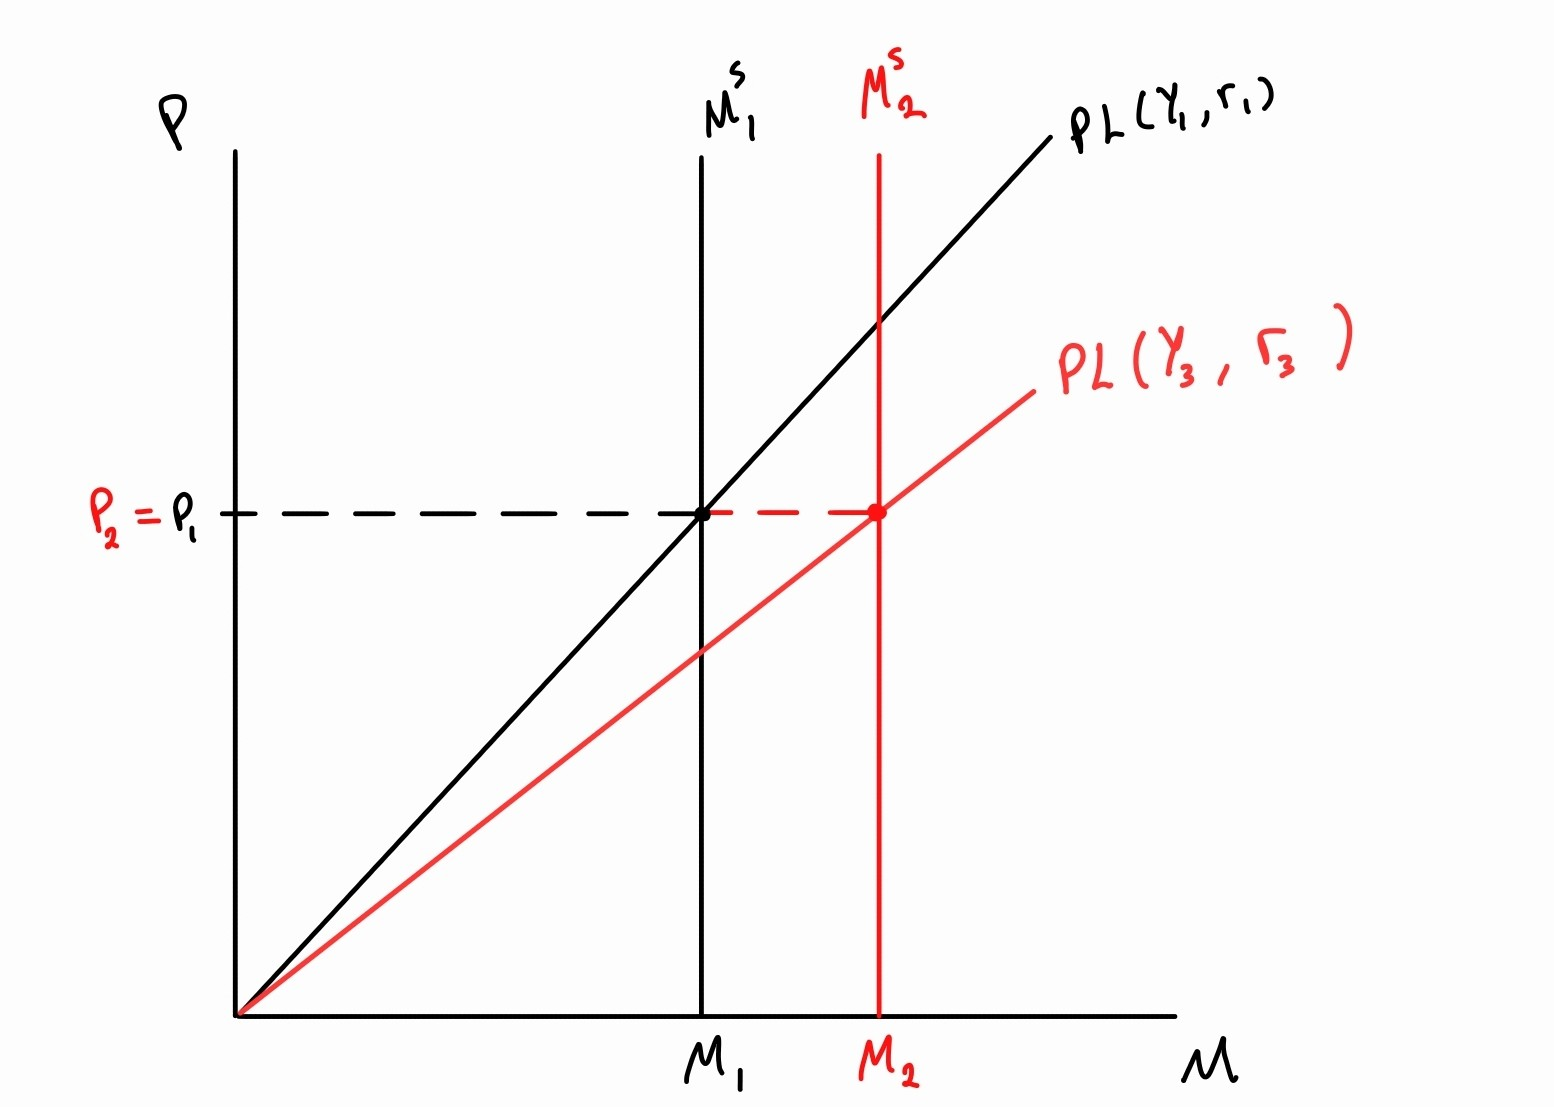
\includegraphics[width=0.75\textwidth]{m2.jpg}
    \caption{Política monetaria con control de la oferta monetaria}
    \label{fig:1.m2}
\end{figure}

Finalmente, dada la neutralidad del dinero en este modelo, el banco central puede realizar los ajustes necesarios en la oferta monetaria para alcanzar su objetivo de inflación sin alterar el equilibrio del sector real de la economía. El nuevo equilibrio en las variables reales permanece determinado exclusivamente por los choques de productividad, independientemente de las decisiones de política monetaria.








\paragraph{Inciso (e).} Supongamos ahora que el banco central utiliza la tasa de interés nominal como objetivo operativo de política monetaria, manteniendo su meta de inflación $\pi^*=0$.

A diferencia del inciso anterior, en el que la tasa de interés nominal se determinaba \textbf{endógenamente} por la ecuación de Fisher, ahora es fijada \textbf{exógenamente} por el banco central. Sin embargo, la ecuación de Fisher debe seguir cumpliéndose en equilibrio. En particular, sabemos que:
\[
1+i=(1+r)(1+\pi).
\]
Utilizando su aproximación de primer orden como igualdad, tenemos que:
\[
i=r+\pi.
\]
Despejando la inflación:
\[
\pi=i-r.
\]
Por lo tanto, para mantener la inflación en su objetivo, el banco central debe ajustar la tasa de interés nominal en la misma dirección y magnitud que los movimientos de la tasa de interés real de equilibrio. En particular:
\begin{align*}
    &\text{Caso (a):}\qquad r_3^a<r_1
    \implies i_3^a<i_1, \\[4pt]
    &\text{Caso (b):}\qquad r_3^b>r_1
    \implies i_3^b>i_1, \\[4pt]
    &\text{Caso (c):}\qquad r_3^c=r_1
    \implies i_3^c=i_1,
\end{align*}
donde $i_1$ representa el nivel inicial de la tasa de política monetaria.

En el escenario (a), el banco central debe reducir su tasa de interés nominal objetivo para acompañar la caída en la tasa de interés real provocada por el choque tecnológico. En el escenario (b), debe incrementarla, dado que el aumento en la demanda de bienes y servicios impulsado por el auge en la inversión eleva la tasa de interés real de equilibrio. Finalmente, en el escenario (c), debe mantenerla constante, pues los efectos de los choques de oferta y demanda sobre la tasa de interés real se compensan exactamente.

Para implementar estas tasas de interés nominales, el banco central debe ajustar la oferta monetaria de manera que el mercado de dinero permanezca en equilibrio. Dado que el objetivo es mantener la inflación en cero, el nivel de precios debe permanecer constante, por lo que la oferta monetaria debe satisfacer:
\[
M_2^x=P_1L(Y_3^x,i_3^x),
\qquad x\in\{a,b,c\}.
\]

En consecuencia, los ajustes requeridos en la oferta monetaria son los mismos que los identificados en el inciso anterior: un incremento en los escenarios (a) y (c), y un ajuste de dirección ambigua en el escenario (b).

Finalmente, dada la neutralidad del dinero en este modelo, los ajustes de política monetaria no tienen repercusiones sobre el equilibrio del sector real. Por lo tanto, el banco central puede acomodar los movimientos de la tasa de interés real mediante ajustes en su tasa nominal objetivo, sin alterar la producción, el consumo, la inversión, el empleo ni las demás variables reales de equilibrio.






\vspace{5em}

\textbf{Ejercicio 3.} En el modelo monetario intertemporal, suponga que el banco central adopta una meta de PIB nominal. Dentro del modelo, esta meta se interpreta como el objetivo de mantener un determinado nivel de PIB nominal constante.
\begin{enumerate}
  \item Suponga un choque positivo permanente en la productividad total de los factores. Dado la meta de política monetaria, ¿qué debe hacer el banco central en respuesta? ¿Cuáles son los efectos sobre las variables agregadas? Explique.

  \item Suponga ahora que ocurre un choque positivo de demanda de dinero. ¿Qué debe hacer el banco central? ¿Cuáles son los efectos sobre las variables agregadas? Explique.
\end{enumerate}




\subsubsection*{Solución.}
Por definición, el PIB nominal es igual al PIB real por el nivel general de precios:
\[
Y^N=PY
\]
Por lo tanto, si el banco central adopta una meta de PIB nominal constante, $Y^N=\bar Y$, debe conducir su política monetaria de manera que:
\[
PY=\bar Y
\]
Esto implica que cualquier variación en la producción real debe ser compensada por una variación proporcional en sentido contrario del nivel general de precios.


\paragraph{Inciso (a).} Un choque positivo permanente en la productividad total de los factores genera los efectos reales analizados en el ejercicio anterior. En particular, independientemente de cuál de los efectos sobre la tasa de interés real domine, la producción agregada aumenta.

Dado que el banco central busca mantener constante el PIB nominal, debe ajustar la oferta monetaria de manera que el incremento en la producción real sea compensado por una reducción en el nivel general de precios. Es decir:
\[
P_1Y_1=P_2Y_3=\bar Y.
\]

Despejando el cambio en el nivel de precios:
\[
\frac{P_2}{P_1}=\frac{Y_1}{Y_3}<1.
\]

Por lo tanto, la inflación debe satisfacer:
\[
\pi=\frac{P_2-P_1}{P_1}
=\frac{Y_1-Y_3}{Y_3}<0.
\]

Es decir, una meta de PIB nominal constante implica que un incremento en la producción real debe estar acompañado de una deflación.

Ahora bien, ¿cómo debe ajustar el banco central la oferta monetaria para alcanzar este resultado? Recordemos que el equilibrio en el mercado de dinero está dado por:
\[
M=PL(Y,i).
\]

Sustituyendo la meta de PIB nominal, $P=\bar Y/Y$, obtenemos:
\[
M=\frac{\bar Y}{Y}L(Y,i).
\]

Para mantener constante el PIB nominal después del choque, la oferta monetaria debe satisfacer:
\[
M_2^x=\frac{\bar Y}{Y_3^x}L(Y_3^x,i_3^x),
\qquad x\in\{a,b,c\}.
\]
Por lo tanto, el crecimiento de la oferta monetaria debe satisfacer:
\[
\frac{M_2^x}{M_1}
=
\frac{Y_1}{Y_3^x}
\frac{L(Y_3^x,i_3^x)}{L(Y_1,i_1)}
\]

En consecuencia, el ajuste requerido en la oferta monetaria depende de la magnitud relativa de los cambios en la producción y en la demanda real de dinero, donde esta última depende de $Y$ y de la tasa de interés. Si esta última aumenta proporcionalmente más que la producción, el banco central debe adoptar una \textbf{política monetaria expansiva}; si aumenta proporcionalmente menos, debe adoptar una \textbf{política contractiva}. Si ambos cambios son proporcionales, la política monetaria debe ser neutral.

\paragraph{Inciso (b).} Supongamos ahora que ocurre un choque positivo en la demanda de dinero. En particular, para cualquier nivel de producción y tasa de interés nominal, los agentes desean mantener una mayor cantidad de saldos monetarios reales.

Dado que se trata de un choque puramente monetario, y por la neutralidad del dinero, el equilibrio del sector real permanece inalterado. En particular:
\[
Y_4=Y_3,
\qquad
r_4=r_3.
\]
donde el subíndice $4$ representa el equilibrio después del choque en el mercado de dinero.

Por lo tanto, para mantener constante el PIB nominal, el banco central debe mantener también constante el nivel general de precios:
\[
P_4Y_4=P_3Y_3=\bar Y.
\]

Como $Y_4=Y_3$, necesariamente:
\[
P_4=P_3.
\]

Sin embargo, el incremento en la demanda real de dinero genera un desequilibrio en el mercado monetario si la oferta nominal de dinero permanece constante. En particular, a los precios y tasas de interés iniciales, la cantidad de dinero que los agentes desean mantener es ahora mayor que la cantidad ofrecida.

Si el banco central no modifica la oferta monetaria, el nivel general de precios tendría que disminuir para restablecer el equilibrio en el mercado de dinero. Dado que la producción real permanece constante, esta reducción en los precios provocaría una caída en el PIB nominal, incumpliendo la meta de política monetaria.

Por lo tanto, el banco central debe incrementar la oferta monetaria para acomodar exactamente el aumento en la demanda real de dinero. Denotando por $L_4$ y $L_3$ las funciones de demanda de dinero antes y después del choque, respectivamente, con:
\[
L_4(Y,i)>L_3(Y,i),
\]
el banco central debe establecer:
\[
M_4=P_3L_3(Y_1,i_1).
\]
Por lo tanto, el crecimiento de la oferta monetaria es:
\[
\boxed{
\frac{M_4}{M_3}
=
\frac{L_4(Y_1,i_1)}{L_3(Y_1,i_1)}>1
}
\]
En consecuencia, el banco central debe incrementar la oferta monetaria exactamente en la misma proporción en que aumenta la demanda real de dinero.


\end{document}